\documentclass{beamer}
\usepackage{amsmath}
\usepackage{amssymb}
\usepackage{gvv}
\usepackage{bm}
\usepackage{graphicx}

\usetheme{Madrid}
\usecolortheme{default}

\title{\textbf{5.3.39}}
\author{\textbf{Aditya Mishra-EE25BTECH11005}}
\date{October 3, 2025}

\begin{document}

\begin{frame}
\titlepage
\end{frame}

\begin{frame}{Question}
Solve the following system of equations:
\[
\begin{cases}
x + y + z = 6 \\
x + 2z = 7 \\
3x + y + z = 12
\end{cases}
\]
\end{frame}

\begin{frame}{Solution}
	Forming Augmented Matrix
\[
\augvec{3}{1}{1 & 1 & 1 & 6 \\ 1 & 0 & 2 & 7 \\ 3 & 1 & 1 & 12}
\]
\end{frame}

\begin{frame}{Solution}
		Row Operations 1
\[
\augvec{3}{1}{1 & 1 & 1 & 6 \\ 1 & 0 & 2 & 7 \\ 3 & 1 & 1 & 12}
\xrightarrow{R_2 \rightarrow R_2 - R_1}
\augvec{3}{1}{1 & 1 & 1 & 6 \\ 0 & -1 & 1 & 1 \\ 3 & 1 & 1 & 12}
\]
\end{frame}

\begin{frame}{Solution}
	Row Operations 2
\[
\augvec{3}{1}{1 & 1 & 1 & 6 \\ 0 & -1 & 1 & 1 \\ 3 & 1 & 1 & 12}
\xrightarrow{R_3 \rightarrow R_3 - 3R_1}
\augvec{3}{1}{1 & 1 & 1 & 6 \\ 0 & -1 & 1 & 1 \\ 0 & -2 & -2 & -6}
\]
\end{frame}

\begin{frame}{Solution}
	Row Operations 3
\[
\augvec{3}{1}{1 & 1 & 1 & 6 \\ 0 & -1 & 1 & 1 \\ 0 & -2 & -2 & -6}
\xrightarrow{R_3 \rightarrow R_3 - 2R_2}
\augvec{3}{1}{1 & 1 & 1 & 6 \\ 0 & -1 & 1 & 1 \\ 0 & 0 & -4 & -8}
\]
\end{frame}

\begin{frame}{Solution}
	Back Substitution
From the third row:
\[
-4z = -8 \implies z = 2
\]

From the second row:
\[
-y + z = 1 \implies -y + 2 = 1 \implies y = 1
\]

From the first row:
\[
x + y + z = 6 \implies x + 1 + 2 = 6 \implies x = 3
\]
\end{frame}

\begin{frame}{Solution}
	The solution of the given system of linear equations is:
\[
\boxed{
\vec{x} = \myvec{3 \\ 1 \\ 2}
}
\]
\end{frame}
\begin{frame}{Plot}
\begin{figure}
    \centering
    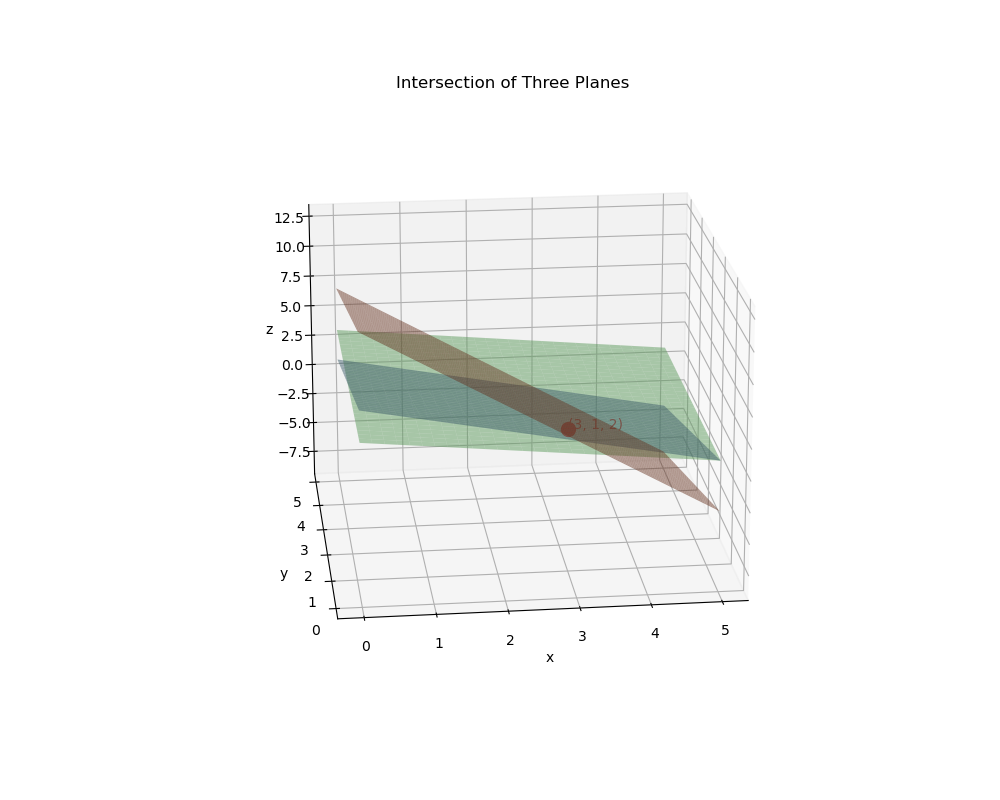
\includegraphics[width=0.8\columnwidth]{Figs/Figure_1.png}
\end{figure}
\end{frame}
\begin{frame}{Codes}
\centering
For Codes, refer to the URL below:  
\url{https://github.com/Aditya-Mishra11005/ee1030-2025/tree/temp/ee25btech11005/matgeo/5.3.39/Codes}
\end{frame}
\end{document}

